%% template for IEICE Transactions
%% v1.8 [2011/12/16]
\documentclass[paper]{ieice}
%\documentclass[invited]{ieice}
%\documentclass[survey]{ieice}
%\documentclass[invitedsurvey]{ieice}
%\documentclass[review]{ieice}
%\documentclass[tutorial]{ieice}
%\documentclass[letter]{ieice}
%\documentclass[brief]{ieice}
\usepackage[dvips]{graphicx}
\usepackage[fleqn]{amsmath}
\usepackage[varg]{txfonts}
\usepackage{subfig}

\setcounter{page}{1}
%\breakauthorline{}% breaks lines after the n-th author

\field{B}
%\SpecialIssue{}
%\SpecialSection{}
%\theme{}
\title{On the Backlog Bound of End-to-End Window Flow Controller}
%\title[title for header]{title}
%\titlenote{This research is supported by High Technology Research and Development Program of China (Grant No. 2012AA012201, 2012AA011902).}
\authorlist{% fill arguments of \authorentry, otherwise error will be caused.
 \authorentry[libaoliang@nudt.edu.cn]{Baoliang LI}{s}{label1}
 \authorentry[zhaojie8037@gmail.com]{Jie ZHAO}{n}{label2}
 \authorentry{Wenhua DOU}{n}{label1}
% \authorentry{name}{membership}{affiliate label}
% \authorentry{name}{membership}{affiliate label}[present affiliate label]
% \authorentry[e-mail address]{name}{membership}{affiliate label}
% \authorentry[e-mail address]{name}{membership}{affiliate label}[present affiliate label]
}
\affiliate[label1]{The authors are with the College of Computer, National University of Defense Technology, China.}
\affiliate[label2]{The author is with the State Key Laboratory of Mathematical Engineering and Advanced Computing, China.}
%\paffiliate[present affiliate label]{Presently, the author is with the }

\received{2014}{01}{8}
%\revised{2014}{01}{8}
%\finalreceived{2011}{1}{1}

%% <local definitions here>

%% </local definitions here>

\newtheorem{theorem}{Theorem}
\newtheorem{lemma}{Lemma}
\newtheorem{definition}{Definition}
\newtheorem{proof}{Proof}

\hyphenation{DNC}
\hyphenation{SNC}
\hyphenation{WFC}
\hyphenation{DCF}

\begin{document}
\maketitle
\begin{summary}
Window Flow Controller (WFC) has been widely used in the computer networks and interconnection networks for its simplicity and high efficiency. In a lossless network with WFC, the unadmitted packets should be blocked and temporarily held by the controller to limit the number of unacknowledged packets in the network. It is very important to quantify the buffer requirement of the WFC, because the buffer is always a scarce resource and should be allocated on demand. In addition, the stochastic backlog bound can also be viewed as the blocking/loss ratio, which is a key Quality-of-Service (QoS) parameter of the network. To meet this great demand, we study the stochastic backlog bound by leveraging the recently developed Stochastic Network Calculus (SNC) theory. Breaking the dependence between arrived traffic and admitted traffic, and characterizing the stochastic backlog bound with stochastic arrival curve of arrived traffic and stochastic service curve provided by the network are the main task of this paper. The main contribution of our work is the derivation of four stochastic backlog bounds for the lossless WFC, with each bound applying under different condition. Our work not only promotes the theory and application of SNC, but also provides a powerful analytical approach for the network performance evaluation and optimization. Experimental results illustrate the tightness and feasibility of our results. %In addition, the impact of different WFC parameters (e.g. offered load, feedback delay and window size) on the backlog bound are also investigated.
\end{summary}
\begin{keywords}
Stochastic Network Calculus, Window Flow Controller, Backlog Bound, feedback network
\end{keywords}

\section{Introduction}
Flow control is an efficient mechanism to avoid network congestion, deadlock and unfair resource allocation \cite{1094691}. Among all these flow control mechanisms, Window Flow Controller (WFC) has been widely used in the computer networks and interconnection networks for its simplicity and high efficiency. The well-known Transmission Control Protocol \cite{RFC5681} and credit-based flow control \cite{372658,DaTo04} are two typical implementations of WFC.\@ In a network with WFC, to realize the lossless transmission, the controller should allocate enough buffer to hold the arrived packets temporarily when the number of unacknowledged packets exceeds the window size.\@ Determining the buffer requirement of lossless WFC is necessary and critical for the following two reasons: (1) The buffer should be allocated on demand, as it is always a scarce resource in any system; (2) The stochastic backlog bound can also be utilized to estimate the blocking/loss ratio for realistic networks, which is a key Quality-of-Service (QoS) parameter. Thus, one question raised: for given WFC parameters, i.e. feedback delay and window size, how to determine the buffer size of the controller under certain arrival and service pattern in order to guarantee certain QoS level? Simulation is commonly used for this purpose, although providing high accuracy, it is very time-consuming and difficult to cover all the configurations. Thus, in this paper, we adopt the analytical approach to evaluate the stochastic backlog bound.

Our theoretical background is the Stochastic Network Calculus (SNC) \cite{Chan94,jiang2006basic,Ciucu2006Scaling,5984844,Fidl06} theory, which has gained great success in the service guarantee of stochastic service systems. Unfortunately, current SNC theory is mainly focusing on the performance analysis of feed-forward network with infinite buffer capacity, and the analysis of feedback network with SNC has been recognized as a research challenge \cite{JiangLiu-15877}. In this paper, we first establish a relationship between the arrival process and the admitted process in idle period, which allows us to use the arrival process and the service process to characterize the backlog bound of WFC. Then, we derive four backlog bounds based on different probability techniques, each with different accuracy and suitable for different scenarios. Our work can be viewed as the stochastic extension of Deterministic Network Calculus (DNC) based WFC performance analysis \cite{CrOk96,AgRa96,Chan98,ACOR99,QLDD09FC,bose2006analysis,Qian2010Analysis}. The obtained results are more general than those obtained by queueing theory, e.g. \cite{1095377,jung1996analysis}, because the latter method restricts the arrival and service to be Markovian. The main contribution of this paper is the derivation of four stochastic backlog bound for the lossless WFC, with each bound applying under different condition. Our work not only extends the application field of SNC to feedback networks, but also provides a novel analytical approach for the performance evaluation of network with feedback control loop. In addition, we also investigated the impact of various WFC parameters (e.g. window size and feedback delay) on the backlog bound.

The rest of this paper is organized as follows. Section \ref{relate} reviews related work. In Section \ref{Notations}, we first introduce the notations and assumptions used in this paper, and then give a brief introduction to the theoretic background of SNC and its related theories. In addition, one method used to obtain the stochastic service curve are also proposed in this Section. The WFC model is introduced in Section \ref{model}. Four backlog bounds are derived in Section \ref{sncloss} with each applying under different conditions. Then, we present the experiment results to verify our results and illustrate the feasibility of our theorems in Section \ref{experiments}. Finally, we summarize this paper in Section \ref{concluson}.

\section{Related Work}\label{relate}
Apart from the simulation based methods, researchers have proposed various analytical methods to analyze the performance of WFC, e.g. queueing theory \cite{1094531,Chu:1981:ATQ:1310158.1310656,berger1992impact,jung1996analysis,1095377,1092752,113869}, automata \cite{Billington:2007:FTD:1366708.1366712}, petri net \cite{Gaeta2003}, max-plus algebra \cite{BaHo00}, control theory \cite{wang2008internet} and DNC \cite{CrOk96,AgRa96,Chan98,ACOR99,QLDD09FC,bose2006analysis,Qian2010Analysis}, etc. For more information about the modeling and analysis of flow and congestion control, please refer to \cite{srikant2004mathematics}. Among all these theories, queueing theory and DNC are the most commonly adopted theories, both achieve great success in the performance modeling and analysis of WFC. Queueing theory is a theory of stochastic service analysis, it mainly focuses on the average performance, e.g. delay, queueing length and utilization, but restricts the arrival and service processes to be Markovian. The most related work to our research is the queueing theory based analysis and optimization of pacing window flow control \cite{jung1996analysis,1095377}, especially the performance model for sliding window flow control proposed in \cite{jung1996analysis}. In the rest of this paper, we will illustrate that, our theorems can provide the same backlog bound as in \cite{jung1996analysis}. Deterministic network calculus is a theory of deterministic queueing system, it mainly focuses on the worst-case performance bound of WFC, e.g. backlog \cite{QLDD09FC,bose2006analysis}, delay \cite{Qian2010Analysis}. However, the worst-case performance bound is very conservative and usually leads to the over-allocation of network resource, because the occurrence of the worst-case scenarios is usually very rare. In addition, just knowing the average or worst-case performance is usually not enough for the guarantee of QoS. Thus, the performance modeling and analysis of WFC still remain an open issue.

In this paper, we fill this gap by leveraging the SNC theory, which is a theory for stochastic service guarantee analysis. Stochastic network calculus is a probabilistic extension of DNC, and gives the performance bound in the manner of probability tail distribution. Although introduced in early 1990s \cite{Chan94}, the theory of SNC becomes applicable recently, and several variations have been proposed, e.g. \cite{jiang2006basic,Fidl06,5984844,Ciucu2006Scaling}. For the systems providing stochastic service, SNC can give more reasonable performance bound than DNC, and be feasible to much more general scenarios than queueing theory. Thus, SNC has been widely used in the field of network coding \cite{10.1109/TPDS.2010.192}, cognitive radio \cite{5466711}, 802.11 DCF \cite{xie2010network}\cite{wang2012effectiveness}, wireless fading channel \cite{Fidler2006network,wangperformance}, etc. Please refer to \cite{JiangLiu-15877} for more details about SNC. However, as far as we know, all these existing applications of SNC are limited to feed-forward networks with infinite buffer capacity. Although the retransmission models in \cite{wangperformance,5466711} introduce the feedback from the destination to the source, the influence of feedback is eliminated by applying either the data scaling element \cite{wangperformance} or the impairment process \cite{5466711}. Our work in this paper is the first attempt to applying the SNC theory directly to the performance analysis of feed-back networks. The derived stochastic backlog bounds compliment the results obtained from queueing theory and DNC.

\section{Preliminaries}\label{Notations}
We first outline the notations used in this paper in Subsection \ref{notation}, then introduce the stochastic arrival curve and stochastic service curve utilized to derive the backlog bounds in Subsection \ref{trafficservice}. Finally, the definition of effective bandwidth and effective capacity are given in Subsection \ref{effectivebandcap}, based on these two concepts, an improved stochastic backlog bound can be obtained.
\subsection{Notations}\label{notation}
In this paper, a process is defined as a non-deceasing casual function on time $t\ (t\geq 0)$. Specifically, denote the accumulative arrival process $\mathcal{A}(t)$ as the amount of traffic (in bits) arrived by time $t$, the accumulative service process $\mathcal{S}(t)$ as the amount of service (in bits) provided by the system by time $t$. Similarly, the accumulative admitted process $\mathcal{I}(t)$ and the accumulative departure process $\mathcal{D}(t)$ denote the amount of traffic entering the system and the amount of traffic departed from the system, respectively. All $\mathcal{A}(t)$, $\mathcal{S}(t)$, $\mathcal{I}(t)$ and $\mathcal{D}(t)$ belong to the set of non-negative non-decreasing functions, denoted by $\mathcal{F}$, and for any function $a(x)\in\mathcal{F}$, let $a(x)=0,\forall x<0$. We also define the following three bivariate functions to simplify our expressions: $\mathcal{A}(s,t)=\mathcal{A}(t)-\mathcal{A}(s)$, $\mathcal{S}(s,t)=\mathcal{S}(t)-\mathcal{S}(s)$ and $\mathcal{D}(s,t)=\mathcal{D}(t)-\mathcal{D}(s)$. The arrival curve and service curve are denoted as $\alpha(t)$ and $\beta(t)$, respectively. The bounding functions of $\alpha(t)$ and $\beta(t)$ are defined as $f(x)$ and $g(x)$, respectively. Without explicit statement, we should always assume that $f(x)$ and $g(x)$ belong to the set of non-negative non-increasing functions, denoted by $\bar{\mathcal{F}}$, and for any function $a(x)\in\bar{\mathcal{F}}$, let $a(x)=1,\forall x<0$. A subset of $\bar{\mathcal{F}}$, denoted by $\bar{\mathcal{G}}$, is defined as, for each function $h(x)\in\bar{\mathcal{G}}$, the $n$th-fold integration, i.e. $(\int_{x}^\infty dy)^nh(y)$, still belongs to $\bar{\mathcal{G}}$. In addition, we leverage the following two notations to shorten our expressions: $[x]_1=\min\{x,1\}$, $[x]^+=\max\{x,0\}$.

The min-plus convolution $\otimes$, deconvolution $\oslash$ and Stieltjes convolution $\ast$ used in this paper are defined as
$$f\otimes g(t)=\min_{0\leq s\leq t}\left\{f(s)+g(t-s)\right\},$$
$$f\oslash g(t)=\sup_{s\geq 0}\left\{f(s+t)-g(s)\right\},$$
$$f\ast g(t)=\int_{-\infty}^{\infty}f(x-y)dg(y).$$

\subsection{Traffic and Service Models}\label{trafficservice}
Stochastic network calculus is developed for the purpose of stochastic performance analysis. Two fundamental concepts in SNC are stochastic arrival curve and stochastic service curve, both have several variations, please refer to \cite{JiangLiu-15877,jiang2006basic} for more details. In order to derive the upper bound of backlog of the controller, we have to adopt the $v.b.c.$ stochastic arrival curve \cite{jiang2006basic,JiangLiu-15877} and $v.b.$ stochastic strict service curve \cite{Wu2010Model} to characterize the traffic and service process, respectively. We only present the definitions of these two models here, because they can be easily found in \cite{JiangLiu-15877,Wu2010Model,jiang2006basic}.

\begin{definition}[$v.b.c.$ stochastic arrival curve]
A flow $\mathcal{A}(t)$ is said to have a virtual-backlog-centric ($v.b.c.$) stochastic arrival curve $\alpha\in\mathcal{F}$ with bounding function $f\in\bar{\mathcal{F}}$, if for all $t\geq 0$ and all $x\geq 0$, the following inequality holds
$$P\left\{\sup_{0\leq s\leq t}\{\mathcal{A}(s,t)-\alpha(t-s)\}>x\right\}\leq f(x).$$
\end{definition}

\begin{definition}[$v.b.$ stochastic strict service curve]
A system $\mathcal{S}(t)$ is said to have a virtual-backlog ($v.b.$) stochastic strict service curve $\beta\in\mathcal{F}$ with bounding function $g\in\bar{\mathcal{F}}$, if for all $x\geq 0$ and $t\geq 0$, the following inequality holds
$$P\left\{\sup_{0\leq s\leq t}\{\beta(t-s)-\mathcal{S}(s,t)\}>x\right\}\leq g(x).$$
\end{definition}

Because the WFC considered in this paper is lossless, thus, in order to keep the system stable, unless explicitly stated, we should always assume the following inequality holds
\begin{equation}
  \lim_{t\to \infty}\frac{1}{t}\left\{\alpha(t)-\beta(t)\right\}\leq 0.
\end{equation}

The $v.b.c.$ stochastic arrival curve has been widely used in SNC to derive performance bound, and several methods have been proposed to obtain this curve, e.g. model transform \cite{jiang2006basic,Wu2010Model,JiangLiu-15877}, queueing theory based method \cite{Wu2010Model} and martingale based method \cite{jiang2010note}. However, methods of obtaining the $v.b.$ stochastic strict service curve are not fully discussed in the literature, because it is only proposed to establish a relationship between queueing theory and stochastic service curve \cite{Wu2010Model}. In this paper, we have to leverage the concept of beginning of last backlogged period to break the dependence between the arrived process and admitted process, and utilize the $v.b.$ stochastic service curve to estimate the backlog bound. Thus, we should first provide some methods which can be used to obtain the $v.b.$ stochastic strict service curve. Apart from the queueing theory based method proposed in \cite{Wu2010Model}, we find that the $v.b.$ stochastic strict service curve has close relationship with stochastic strict service curve \cite{JiangLiu-15877}. So, we propose a model transform based method, i.e. Theorem \ref{mtrans}, to obtain the $v.b.$ stochastic strict service curve from stochastic strict service curve.
\begin{theorem}\label{mtrans}
(1) If a system $\mathcal{S}(t)$ provides a $v.b.$ stochastic strict service curve $\beta(t)\in\mathcal{F}$ with bounding function $g(x)\in\bar{\mathcal{F}}$, the system also provides a stochastic strict service curve with the same service curve and bounding function.

(2) If a system $\mathcal{S}(t)$ provides a stochastic strict service curve $\beta(t)\in\mathcal{F}$ with bounding function $g(x)\in\bar{\mathcal{G}}$ and $\beta_{\theta}(t)=\beta(t)-\theta\cdot t\in\mathcal{F}$ for some $\theta>0$, it also provides a $v.b.$ stochastic strict service curve $\beta_{\theta}(t)$ with bounding function $g_{\theta}(x)=[g(x)+\frac{1}{\theta}\int_x^\infty g(y)dy]_1$ for any $\theta>0$ satisfying $\beta_{\theta}(t)\in\mathcal{F}$.
\end{theorem}

\begin{proof}
(1) Obviously, for any $0\leq s\leq t$, we have
$$\beta(t-s)-\mathcal{S}(s,t)\leq \sup_{0\leq s^\prime\leq t}\left\{\beta(t-s^\prime)-\mathcal{S}(s^\prime,t)\right\}$$
which implies the following inequality
\begin{eqnarray*}
\lefteqn{P\left\{\beta(t-s)-\mathcal{S}(s,t)>x\right\}}\\
&\leq& P\left\{\sup_{0\leq s^\prime\leq t}\left\{\beta(t-s^\prime)-\mathcal{S}(s^\prime,t)\right\}>x\right\}.
\end{eqnarray*}
The left side of this inequality corresponds to the stochastic strict service curve. Thus, the bounding function of $v.b.$ stochastic strict service curve is indeed a bounding function for the stochastic strict service curve with the same stochastic strict service curve.

(2) If a system $\mathcal{S}(t)$ provides a stochastic strict service curve $\beta(t)$ with bounding function $g\in\bar{\mathcal{G}}$, and $\beta(t)-\theta \cdot t\in\mathcal{F}$, where $\theta>0$ is a free parameter, then, for any $\theta$ satisfying $\beta_{\theta}(t)\in\mathcal{F}$, we can construct a $v.b.$ stochastic strict service curve $\beta_{\theta}(t)=\beta(t)-\theta \cdot t$. The bounding function of $\beta_\theta(t)$ can be obtained following the same procedure of Theorem 3.13 in \cite{JiangLiu-15877}, which is
\begin{eqnarray*}
\lefteqn{P\left\{\sup_{0\leq s\leq t}\{\beta_{\theta}(t-s)-\mathcal{S}(s,t)\}>x\right\}}\\
&\leq &\sum_{s=0}^t P\left\{[\beta_{\theta}(t-s)-\mathcal{S}(s,t)]^+>x\right\}\\
&\leq &\sum_{s=0}^t g(x+\theta\cdot(t-s))\\
&\leq & \sum_{\tau=0}^\infty g(x+\theta\tau)\\
&\leq & g(x)+\frac{1}{\theta}\int_{x}^\infty g(y)dy
\end{eqnarray*}
which completes the proof.\QED
\end{proof}

\subsection{Effective Bandwidth and Effective Capacity}\label{effectivebandcap}
Stochastic network calculus utilizes stochastic arrival curve and stochastic service curve to describe the arrival and service process, and derive the performance bound based on some basic probability techniques. It usually does not make any assumption on the arrival and service processes, making it feasible to wide range of applications. However, for some specific conditions, much tighter bound can be obtained if some advance probability techniques, e.g. effective bandwidth, effective capacity and martingale theory can be integrated into the analysis framework, e.g. \cite{Li2007Network,5984844,jiang2009network,Ciucu2007Network}. Here, we present the concepts of effective bandwidth \cite{Kelly1996Note} and effective capacity \cite{Wu2003Effective} used in this paper to derive the backlog bound for stationary arrival and service processes.
\begin{definition}[Effective Bandwidth and Effective Capacity]
For all $\theta_a>0$ and $t_a<\infty$, the effective bandwidth with respect to a flow is defined as
$$\rho(\theta_a,t_a)=\frac{1}{\theta_a t_a}log E[e^{\theta_a \mathcal{A}(t_a)}]$$
where the parameters $\theta_a$ and $t_a$ are called the space parameter and time parameter, respectively. Similarly, for all $\theta_s>0$ and $t_s>0$, the effective capacity of service process $\mathcal{S}(t_s)$ is defined as
$$\mu^\prime(\theta_s,t_s)=\frac{1}{-\theta_s t_s}log E[e^{-\theta_s \mathcal{S}(t_s)}]$$
where the parameters $\theta_s$ and $t_s$ are called space parameter and time parameter, respectively.
\end{definition}

For a lossless system described with effective bandwidth and effective capacity, the following stability condition should be hold for $\forall t>0$,
$$\rho(\theta,t)\leq \mu^\prime(\theta,t).$$

\section{Network Model}\label{model}
Flow control is an efficient solution for the networks to prevent the sender from overflowing the buffer of the receiver. In the computer networks, a packet/frame flow generated by a source traverses several intermediate nodes (e.g. switch or router) and terminated at the destination. To prevent buffer overflow, the number of packets/frame \textquoteleft in flight\textquoteright\ should be limited. This is achieved by enforcing the destination return an acknowledgment to the source for each packet/frame correctly received. The source releases a packet/frame whenever the number of unacknowledged packet/frame does not exceed the window size $W$. Apart from the TCP \cite{RFC5681} in transmission layer, two typical flow control mechanisms in data link layer, i.e. sliding window and stop-and-wait, can also be viewed as window flow control, corresponding to the $W>1$ and $W=1$ scenarios. Credit-based flow control is another example of WFC, it maintains a counter at the sender to track the buffer available at the receiver. This counter increases when the receiver consumes a cell and decreases when the sender releases a cell.

The closed-loop flow control mechanism discussed above has been deeply investigated with DNC \cite{CrOk96,AgRa96,Chan98,ACOR99,QLDD09FC,bose2006analysis,Qian2010Analysis}, as illustrated in Fig. \ref{control}. This model is comprised of two sub-systems in tandem, and the second sub-system has finite buffer capacity. The number of acknowledgements feed back to the source by time $t$ is denoted as $\mathcal{D}(t-\tau)$, where $\tau$ is the feedback delay. If the amount of traffic unacknowledged at time instance $t$ is less than the maximal window size $W$, the traffic arrived at the first sub-system can be departed and injected into second sub-system immediately, or else, stays in the first sub-system to ensure that the amount of unacknowledged traffic never exceeds $W$. Services offered to the admitted flow, $\mathcal{S}(t)$, can be obtained by subtracting the total service capacity provided by the network from the services consumed by the inference traffic. To simplify our discussion, suppose all the acknowledgements feed back from the destination experience the same delay $\tau$. The accumulative admitted process $\mathcal{I}(t)$ satisfies
\begin{equation}\label{wfc}
\mathcal{I}(t)=\min\{\mathcal{A}(t),\mathcal{D}(t-\tau)+W\}.
\end{equation}
\begin{figure}[ht]
  \centering\includegraphics[scale=0.45]{figures/QueueModel.eps}\\
  \caption{End-to-End Flow Control}\label{control}
\end{figure}

We must claim that, although the model presented here is much simpler than the flow control in realistic networks, it is sufficient to demonstrate the key design consideration and the necessary tradeoff that should be made. The backlog of controller at time $t$ can be expressed as:
$$\mathcal{L}(t)=\mathcal{A}(t)-\mathcal{I}(t).$$
And the backlog bound $P\{\mathcal{L}(t)>x\}$ is the probability upper bound that the backlog in the controller at time instance $t$ is greater than $x$. This performance metric is important for the allocation of buffer and the analysis of buffer utilization. Actually, this upper bound can also be viewed as the blocking/loss ratio of this system. In addition, if $\tau=0$ and $W=0$ in our model, $P\{\mathcal{L}(t)>x\}$ is the same as the backlog bound of feed-forward system with arrival process $\mathcal{A}(t)$ and service process $\mathcal{S}(t)$. Unfortunately, deriving the backlog bound is a non-trival task, this is because there exists dependence between $\mathcal{I}(t)$ and $\mathcal{A}(t)$, as shown in Eq.(\ref{wfc}).

\section{Backlog Bound of Window Flow Controller}\label{sncloss}
In this section, we will take up the challenge to derive stochastic backlog bound for the lossless WFC. The backlog bound of the WFC is closely related with the window size, service rate, arrival rate and feedback delay, etc. which makes the modeling and analysis very difficult and complex. We first list the necessary Lemmas in Subsection \ref{neclemma}. Based on these Lemmas, we derive four backlog bounds for the WFC in Subsection \ref{backlog}.
\subsection{Necessary Lemmas}\label{neclemma}
The following two Lemmas will be used in our derivation to evaluate the tail distribution of random variables. These two Lemmas have been verified in \cite{jiang2006basic}.
\begin{lemma}\label{lamma1}
For any random variable $X$ and any real number $x\geq 0$, we have $$P\{[X]^+>x\}=P\{X>x\}.$$
\end{lemma}

\begin{lemma}\label{lamma3}
For any two random variables $X$ and $Y$, and any real number $x\geq 0$, there holds
$$P\{X+Y>x\}\leq f\otimes g(x)$$
if $P\{X>x\}\leq f(x)$, $P\{Y>x\}\leq g(x)$ and $f(x),g(x)\in\bar{\mathcal{F}}$.

Furthermore, if $X$ and $Y$ are independent, there holds
$$P\left\{X+Y>x\right\}\leq 1-\bar{f}\ast\bar{g}(x)$$
where $\bar{f}(x)=1-[f(x)]_1$ and $\bar{g}(x)=1-[g(x)]_1$.
\end{lemma}

The following Lemma establishes the relationship between the admitted process and the arrival process in idle period, which serves as the basis for our further derivation.
\begin{lemma}[Flow Control Principle]\label{lama1}
If $t_0$ is in one of the idle period of lossless WFC shown in Fig. \ref{control}, $\mathcal{A}(t)$ and $\mathcal{I}(t)$ are the arrival process and admitted process, respectively. Then, for a sufficient short feedback delay $\tau$, we have
\begin{equation}
\mathcal{I}(t_0)=\mathcal{A}(t_0).
\end{equation}
\end{lemma}
\begin{proof}
Obviously, for $\forall t\geq 0$, $\mathcal{I}(t)\leq \mathcal{A}(t)$ for casuality. At time instance $t_0$, if $\mathcal{I}(t_0)<\mathcal{A}(t_0)$, buffered data in controller will be admitted and makes the WFC keep on working (this is because the feedback delay is sufficient short), which is contrary to the fact that $t_0$ is in the idle period. Thus, $\mathcal{I}(t_0)=\mathcal{A}(t_0)$.\QED
\end{proof}

Based on Lemma \ref{lama1}, we can get the follow Lemma. This Lemma makes no assumptions on the arrival process and service process, and serves as the basis to derive all the four backlog bounds in Subsection \ref{backlog}.
\begin{lemma}\label{lama2}
Let $\mathcal{A}(t)$ and $\mathcal{D}(t)$ be the arrival process and departure process, $\tau$ and $W$ be the feedback delay and window size. Then, the backlog bound in the controller satisfies
$$P\{\mathcal{L}(t)>x\}=P\{\mathcal{A}(t)-\mathcal{D}(t-\tau)-W>x\}.$$
\end{lemma}
\begin{proof}
As shown in Fig. \ref{control}, for any sample path $\mathcal{A}(t)$ and $\mathcal{D}(t)$, the backlog $\mathcal{L}(t)$ in WFC can be expressed as
\begin{eqnarray}
  \mathcal{L}(t)&=&\mathcal{A}(t)-\mathcal{I}(t)\nonumber\\
      &=&\mathcal{A}(t)-\min\{\mathcal{A}(t),\mathcal{D}(t-\tau)+W\}\nonumber\\
      &=&[\mathcal{A}(t)-\mathcal{D}(t-\tau)-W]^+.\nonumber
\end{eqnarray}

Thus, according to Lemma \ref{lamma1}, we have
\begin{eqnarray*}
  P\{\mathcal{L}(t)>x\}&=&P\{[\mathcal{A}(t)-\mathcal{D}(t-\tau)-W]^+>x\}\\
  &=&P\{\mathcal{A}(t)-\mathcal{D}(t-\tau)-W>x\}.
\end{eqnarray*}
which ends the proof.\QED
\end{proof}

The following lemma will be used to obtain the backlog bound when the $\mathcal{A}(t)$ and $\mathcal{S}(t)$ are stationary\footnote{The special case of this Lemma, i.e. $\tau=0$, has been proposed in \cite{5984844} to derive the performance bounds of feed-forward networks.}.
\begin{lemma}\label{lama3}
Suppose stochastic process $\mathcal{A}(t)$ and $\mathcal{S}(t)$ are both stationary process. Let $\eta$ be the first time instance that stochastic process $\{\mathcal{A}(t)-\mathcal{S}(t-\tau),t\geq \tau\}$ is greater than or equal to a positive real number $x$ in the interval $[\tau,\infty]$. Then
$$P\{\sup_{0\leq s\leq t-\tau}\{\mathcal{A}(s,t)-\mathcal{S}(s,t-\tau)\}>x\}=P\{\tau\leq \eta<\infty\}.$$
\end{lemma}
\begin{proof}
Because stochastic process $\mathcal{A}(t)$ and $\mathcal{S}(t)$ are both stationary process, we have
\begin{eqnarray*}
\lefteqn{P\{\sup_{0\leq s\leq t-\tau}\{\mathcal{A}(s,t)-\mathcal{S}(s,t-\tau)\}>x\}}\\
&=&P\{\sup_{\tau\leq u\leq t}\{\mathcal{A}(u)-\mathcal{S}(u-\tau)\}>x\}\\
&\leq&P\{\sup_{u\geq \tau}\{\mathcal{A}(u)-\mathcal{S}(u-\tau)\}>x\}.
\end{eqnarray*}

Denote by $\eta$ ($\eta\geq \tau$) the first time instance that stochastic process $\{\mathcal{A}(t)-\mathcal{S}(t-\tau),t\geq \tau\}$ is greater than or equal to a positive real number $x$. If $\eta<\infty$, we have
$$x\leq \{\mathcal{A}(\eta)-\mathcal{S}(\eta-\tau)\}\leq \sup_{u\geq \tau}\{\mathcal{A}(u)-\mathcal{S}(u-\tau)\}.$$
In other words, event $\{\tau\leq \eta<\infty\}$ implies event $\{\sup_{u\geq \tau}\{\mathcal{A}(u)-\mathcal{S}(u-\tau)\}>x\}$.

On the other hands, if $\sup_{u\geq \tau}\{\mathcal{A}(u)-\mathcal{S}(u-\tau)\}>x$, there must exists some $\eta\in[\tau,\infty)$ satisfying $\mathcal{A}(\eta)-\mathcal{S}(\eta-\tau)\geq x$, then the minimum $\eta$ is the first time instance which makes $\mathcal{A}(u)-\mathcal{S}(u-\tau)$ greater than or equal to $x$. In other words, event $\{\sup_{u\geq \tau}\{\mathcal{A}(u)-\mathcal{S}(u-\tau)\}>x\}$ implies $\{\tau\leq\eta<\infty\}$.

Combining these two cases, we get
$$P\{\sup_{0\leq s\leq t-\tau}\{\mathcal{A}(s,t)-\mathcal{S}(s,t-\tau)\}>x\}=P\{\tau\leq\eta<\infty\}$$
which ends the proof.\QED
\end{proof}

The following Lemma is utilized to derive the exact backlog bound for the independent and stationary increment arrival and service process, please refer to \cite{jiang2009network,Ciucu2007Network} for the proof of this Lemma.
\begin{lemma}\label{lamma5}
Suppose $\mathcal{A}(t)$ and $\mathcal{S}(t)$ both have independent and stationary increments, $\theta>0$ is a free parameter. For fixed $t\geq 0$, let $U_{t}(v)=e^{\theta[\mathcal{A}(t-v,t)-\mathcal{S}(t-v,t)]}$, if $E[e^{\theta (\mathcal{A}(1)-\mathcal{S}(1))}]\leq 1$, stochastic process $\left\{U_{t}(v),1\leq v\leq t\right\}$ is a supermartingale.
\end{lemma}

\subsection{Backlog Bound}\label{backlog}
In this Subsection, we will try to break the dependence between arrived traffic $\mathcal{A}(t)$ and admitted traffic $\mathcal{I}(t)$, and provide four backlog bounds for the WFC, each with different applying condition.
\begin{theorem}[Backlog Bound for WFC]\label{theorem1}
For a WFC with feedback delay $\tau$ and window size $W$, if the arrival process and service process are $\mathcal{A}(t)$ and $\mathcal{S}(t)$, respectively. Suppose the arrival process $\mathcal{A}(t)$ has a $v.b.c.$ stochastic arrival curve $<f,\alpha>$, service process $\mathcal{S}(t)$ has a $v.b.$ stochastic strict service curve $<g,\beta>$, then, the backlog $\mathcal{L}(t)$ in the WFC is bounded by
\begin{equation}\label{eqn1}
P\left\{\mathcal{L}(t)>x\right\}\leq [f\otimes g([x+W-\alpha\oslash\beta(\tau)]^+)]_1.
\end{equation}

If $\mathcal{A}(t)$ and $\mathcal{S}(t)$ are independent, we can get a much tighter backlog bound with Stieljes convolution
\begin{equation}\label{eqn2}
P\{\mathcal{L}(t)>x\}\leq 1-\bar{f}\ast\bar{g}([x+W-\alpha\oslash\beta(\tau)]^+).
\end{equation}
\end{theorem}

\begin{proof}
Inspired by Lemma \ref{lama2}, to evaluate $P\{\mathcal{L}(t)>x\}$, we can estimate $P\{\mathcal{A}(t)-\mathcal{D}(t-\tau)-W>x\}$ first.

Denote $t_{0}$ is the beginning of last backlogged period before $t-\tau$, i.e. let $t_0=\sup\{s\in[0,t-\tau]:\mathcal{I}(s)=\mathcal{D}(s)\}$ \cite{Fidl06}, then $0\leq t_{0}\leq t-\tau$. We have
\begin{eqnarray*}
  \mathcal{D}(t-\tau)&=&\mathcal{I}(t_{0})+\mathcal{S}(t_{0},t-\tau)\\
  &=& \mathcal{A}(t_{0})+\mathcal{S}(t_{0},t-\tau).
\end{eqnarray*}

Hence,
\begin{eqnarray*}
P\{\mathcal{L}(t)>x\}&=&P\{\mathcal{A}(t)-\mathcal{D}(t-\tau)-W>x\}\\
&=&P\{\mathcal{A}(t_0,t)-\mathcal{S}(t_0,t-\tau)-W>x\}.
\end{eqnarray*}

Now, we have broken the dependence between $\mathcal{I}(t)$ and $\mathcal{A}(t)$. But, the obtained probability bound is a conditional probability, because $t_{0}$ is a random variable. To estimate the conditional probability bound, let
\begin{eqnarray}\label{condprob}
\lefteqn{\mathcal{A}(t_0,t)-\mathcal{S}(t_0,t-\tau)-W}\nonumber\\
&=&[\mathcal{A}(t_{0},t)-\alpha(t-t_{0})]-W\nonumber\\
&&+[\beta(t-\tau-t_{0})-\mathcal{S}(t_{0},t-\tau)]\nonumber\\
&&+[\alpha(t-t_{0})-\beta(t-\tau-t_{0})].
\end{eqnarray}

For the expression in the last square brackets, let $s=t-t_{0}-\tau$, thus $0\leq s\leq t-\tau$, and
\begin{eqnarray}\label{curve}
  \alpha(t-t_{0})-\beta(t-\tau-t_{0})&\leq &\sup_{0\leq s\leq t-\tau}\{\alpha(s+\tau)-\beta(s)\}\nonumber\\
  &\leq & \alpha\oslash\beta(\tau).
\end{eqnarray}

Denote by $\mathcal{X}(t)=\sup_{0\leq s\leq t}\{\mathcal{A}(s,t)-\alpha(t-s)\}$ and $\mathcal{Y}(t)=\sup_{0\leq s\leq t-\tau}\{\beta(t-\tau-s)-\mathcal{S}(s,t-\tau)\}$, we have
\begin{equation}\label{vbc}
\mathcal{A}(t_{0},t)-\alpha(t-t_{0})\leq \mathcal{X}(t),
\end{equation}
\begin{equation}\label{vb}
\beta(t-\tau-t_{0})-\mathcal{S}(t_{0},t-\tau)\leq \mathcal{Y}(t).
\end{equation}

Bringing Eq.(\ref{curve}), Eq.(\ref{vbc}) and Eq.(\ref{vb}) into Eq.(\ref{condprob}), we get
$$\mathcal{A}(t_0,t)-\mathcal{S}(t_0,t-\tau)-W \leq \mathcal{X}(t)+\mathcal{Y}(t)+\alpha\oslash\beta(\tau)-W.$$

This inequality is sufficient to obtain the upper bound of $P\{\mathcal{A}(t_0,t)-\mathcal{S}(t_0,t-\tau)-W>x\}$, because event $\{\mathcal{A}(t_0,t)-\mathcal{S}(t_0,t-\tau)-W>x\}$ implies $\{\mathcal{X}(t)+\mathcal{Y}(t)+\alpha\oslash\beta(\tau)-W\}$. Thus, we have
$$P\{\mathcal{A}(t_0,t)-\mathcal{S}(t_0,t-\tau)-W>x\}\leq P\{\mathcal{X}(t)+\mathcal{Y}(t)>y^\prime\}$$
where $y^\prime=x+W-\alpha\oslash\beta(\tau)$.

We also notice that, we can provide a bound for $P\{\mathcal{X}(t)+\mathcal{Y}(t)>y^\prime\}$ by leveraging Lemma \ref{lamma3}. Because $P\{\mathcal{X}(t)>y^\prime\}$ and $P\{\mathcal{Y}(t)>y^\prime\}$ are closely related to the $v.b.c.$ stochastic arrival curve and $v.b.$ stochastic strict service curve, respectively. But, we have to consider the following two cases according to the value of $y^\prime$.

(1) $y^\prime\geq 0$. Based on the definition of $v.b.c.$ stochastic arrival curve and $v.b.$ stochastic strict service curve, we get
$$P\{\mathcal{X}(t)>y^\prime\}\leq f(y^\prime),$$
$$P\{\mathcal{Y}(t)>y^\prime\}\leq g(y^\prime).$$

By applying Lemma \ref{lamma3}, we have
\begin{equation}\label{equation1}
P\{\mathcal{X}(t)+\mathcal{Y}(t)>y^\prime\}\leq f\otimes g(y^\prime).
\end{equation}

(2) $y^\prime<0$. Because $\mathcal{X}(t)\geq 0$ and $\mathcal{Y}(t)\geq 0$, we have
$$P\{\mathcal{X}(t)>y^\prime\}=P\{\mathcal{X}(t)>0\}\leq f(0).$$
$$P\{\mathcal{Y}(t)>y^\prime\}=P\{\mathcal{Y}(t)>0\}\leq g(0).$$

Thus,
\begin{equation}\label{equation2}
P\{\mathcal{X}(t)+\mathcal{Y}(t)>y^\prime\}\leq f\otimes g(0).
\end{equation}

Combining these two cases, we have
\begin{eqnarray*}
  P\{\mathcal{L}(t)>x\}&=&P\{\mathcal{A}(t)-\mathcal{D}(t-\tau)-W>x\}\\
  &\leq&P\{\mathcal{X}(t)+\mathcal{Y}(t)>y^\prime\}\\
  &\leq& f\otimes g([y^\prime]^+).
\end{eqnarray*}

If $\mathcal{A}(t)$ and $\mathcal{S}(t)$ are independent, we can adopt the Stieltjes convolution to get a much tighter probability bound
$$P\{\mathcal{L}(t)>x\}\leq 1-\bar{f}\ast\bar{g}([y^\prime]^+)$$
which ends the proof.\QED
\end{proof}

The above theorem was derived based on some basic probability techniques without making any assumption on the arrival process and service process. Although generality, the backlog bound can be further improved if we take the characterization of arrival and service into consideration. As shown in the following two theorems.

\begin{theorem}\label{theorem2}
For a WFC with feedback delay $\tau$ and window size $W$, if the arrival process and service process are $\mathcal{A}(t)$ and $\mathcal{S}(t)$, respectively. If $\mathcal{A}(t)$ and $\mathcal{S}(t)$ are both stationary processes, the backlog bound is
\begin{eqnarray*}\label{eqn4}
P\{\mathcal{L}(t)>x\}&\leq& \inf_{\theta\in \Theta}\{e^{\theta(\sup_{u\geq \tau}\{u\alpha(\theta,u)-(u-\tau)\beta(\theta,u-\tau)\}-W-x)}\}.
\end{eqnarray*}
where $\Theta$ is the set of $\theta$ satisfying $\alpha(\theta,t)\leq \beta(\theta,t)$.
\end{theorem}

\begin{proof}
Denote by $\eta$ the first time instance that satisfies $\mathcal{A}(t)-\mathcal{S}(t-\tau)\geq W+x$. Then
\begin{eqnarray}\label{effective1}
  \lefteqn{E[e^{\theta(\mathcal{A}(\eta)-\mathcal{S}(\eta-\tau))}]}\nonumber\\
  &=&E[e^{\theta(\mathcal{A}(\eta)-\mathcal{S}(\eta-\tau))}|\tau\leq\eta<\infty]\cdot P\{\tau\leq \eta<\infty\}\nonumber\\
  &&+E[e^{\theta(\mathcal{A}(\eta)-\mathcal{S}(\eta-\tau))}|\eta=\infty]\cdot P\{\eta=\infty\}\nonumber\\
  &\geq& E[e^{\theta(\mathcal{A}(\eta)-\mathcal{S}(\eta-\tau))}|\tau\leq\eta<\infty]\cdot P\{\tau\leq \eta<\infty\}\nonumber\\
  &\geq& e^{\theta (W+x)}\cdot P\{\tau\leq \eta<\infty\}.
\end{eqnarray}
The last inequality holds because $\eta$ is the first time instance satisfying $\mathcal{A}(\eta)-\mathcal{S}(\eta-\tau)>W+x$, then
$E[e^{\theta(\mathcal{A}(\eta)-\mathcal{S}(\eta-\tau))}|\{\tau\leq\eta<\infty\}]\geq e^{\theta (W+x)}$.

On the other hands, if $\mathcal{A}(t)$ and $\mathcal{S}(t)$ are both stationary increments processes, based on the definition of effective bandwidth and effective capacity, we have\footnote{The special case of this inequality, i.e. $\tau=0$, has been proposed in \cite{5984844} for the feed-forward networks.}
\begin{eqnarray}\label{effective2}
E[e^{\theta(\mathcal{A}(\eta)-\mathcal{S}(\eta-\tau))}]&=&e^{\theta(\eta\alpha(\theta,\eta)-\beta(\theta,\eta-\tau))}\nonumber\\
&\leq& e^{\theta\sup_{u\geq \tau}(u\alpha(\theta,u)-(u-\tau)\beta(\theta,u-\tau))}.
\end{eqnarray}

Combining Eq.(\ref{effective1}) and Eq.(\ref{effective2}), we have
$$e^{\theta (W+x)}\cdot P\{\tau\leq\eta<\infty\}\leq e^{\theta\sup_{u\geq \tau}(u\alpha(\theta,u)-(u-\tau)\beta(\theta,u-\tau))}.$$

By applying Lemma \ref{lama2} and Lemma \ref{lama3}, we get
\begin{eqnarray*}
\lefteqn{P\{\mathcal{L}(t)>x\}}\\
&=&P\{\mathcal{A}(t)-\mathcal{D}(t-\tau)-W>x\}\\
&=&P\{\mathcal{A}(t_0,t)-\mathcal{S}(t_0,t-\tau)-W>x\}\\
&\leq&P\{\sup_{0\leq s\leq t-\tau}\{\mathcal{A}(s,t)-\mathcal{S}(s,t-\tau)\}>W+x\}\\
&=&P\{\tau\leq \eta<\infty\}\\
&\leq& e^{-\theta (W+x)}\cdot e^{\theta\sup_{u\geq \tau}\{u\alpha(\theta,u)-(u-\tau)\beta(\theta,u-\tau)\}}.
\end{eqnarray*}
which ends the proof.\QED
\end{proof}

\begin{theorem}\label{theorem3}
For a WFC with feedback delay $\tau$ and window size $W$, if the arrival process and service process are $\mathcal{A}(t)$ and $\mathcal{S}(t)$, respectively. If $\mathcal{A}(t)$ and $\mathcal{S}(t)$ are independent and stationary increments and $\tau=0$, an exact distribution of backlog can be obtained by leverage the Doob's martingale inequality
\begin{equation}\label{eqn3}
P\left\{\mathcal{L}(t)>x\right\}\leq \inf_{\theta\in\Theta}\{e^{-\theta(W+x)}\cdot E[e^{\theta(\mathcal{A}(1)-\mathcal{S}(1))}]\}.
\end{equation}
where $\Theta$ is the set of $\theta$ satisfying $E[e^{\theta(\mathcal{A}(1)-\mathcal{S}(1))}]\leq 1$.
\end{theorem}
\begin{proof}
If arrival process $\mathcal{A}(t)$ and service process $\mathcal{S}(t)$ are independent and stationary increments process, and feedback delay $\tau=0$, according to Lemma \ref{lamma5}, we know that when $E[e^{\theta(\mathcal{A}(1)-\mathcal{S}(1))}]\leq 1$, stochastic process $\{U_{t}(v),1\leq v\leq t\}$ is a supermartingale, then, following the same procedure in \cite{Ciucu2007Network}\cite{jiang2009network}, we have
\begin{eqnarray*}
P\left\{\mathcal{L}(t)>x\right\}  &=&P\left\{\mathcal{A}(t_{0},t)-\mathcal{S}(t_{0},t)-W>x\right\}\\
  &\leq& P\left\{\sup_{0\leq s\leq t}\{\mathcal{A}(s,t)-\mathcal{S}(s,t)\}>W+x\right\}\\
  &=& P\left\{\sup_{0\leq s< t}e^{\theta\{\mathcal{A}(s,t)-\mathcal{S}(s,t)\}}>e^{\theta(W+x)}\right\}\\
  &=& P\left\{\sup_{1\leq v\leq t}e^{\theta\{\mathcal{A}(t-v,t)-\mathcal{S}(t-v,t)\}}>e^{\theta(W+x)}\right\}\\
  &=& P\left\{\sup_{1\leq v\leq t}U_{t}(v)>e^{\theta(W+x)}\right\}\\
  &\leq& e^{-\theta(W+x)}\cdot E[U_{t}(1)]\\
  &=& e^{-\theta(W+x)}\cdot E[e^{\theta(\mathcal{A}(1)-\mathcal{S}(1))}].
\end{eqnarray*}

We can optimize the backlog bound by free parameter $\theta$ satisfying $E[e^{\theta(\mathcal{A}(1)-\mathcal{S}(1))}]\leq 1$.\QED
\end{proof}

\section{Experiment Results}\label{experiments}
In this section, we present the numerical results of backlog bounds calculated with our theorems, and compare them with the simulation results. To get the simulation results, we built an event-driven simulator based on the OMNeT++ discrete-event simulation platform \cite{omnetpp}. Our goals in this section are three-folded: (1) We try to demonstrate the feasibility of our theorems and the tightness of our results by comparing with the simulation results; (2) We want to show that, our results are more general than the backlog bound proposed in \cite{jung1996analysis}; (3) We intend to illustrate the impact of different offered load and window control parameters, i.e. window size and feedback delay on the backlog bound of WFC. To achieve these goals, three arrival and service processes combinations are considered in this section: (1) Scenario I: Poisson input and constant rate service; (2) Scenario II: Poisson input with exponentially distributed service time, and the feedback delay $\tau=0$; (3) Scenario III: Bernoulli input and exponentially distributed service time. The reason of choosing these three models is that, there already exists extensive research results for these arrival and service model, which can be directly used to derive our backlog bounds.

\subsection{Backlog Bound for Scenario I}
Suppose all the packets in the traffic flow have the same length $L$, and the packet arrivals subject to Poisson process with parameter $\lambda$. Then, the traffic has a $v.b.c.$ stochastic arrival curve $<e^{-\theta_1^\prime\theta_1}e^{-\theta_1 x},\frac{\lambda}{\theta_1}(e^{\theta_1 L}-1)\cdot t+\theta_1^\prime\cdot t>$ \cite{jiang2010note}, where $\theta_1\geq 0$ and $\theta>0$ are free parameters. We can also easily verify that the constant rate server provides a $v.b.$ stochastic strict service curve $<0,C\cdot [t-0]^+>$, where $C$ is the service rate.

Let $\theta_1^\prime=0$, we can get the backlog bound with Eq.(\ref{eqn2}), which is
\begin{eqnarray}\label{bounding}
P\{\mathcal{L}(t)>x\}&\leq& f([x+W-\alpha\oslash\beta(\tau)]^+)\}\nonumber\\
&=& e^{-\theta_1([x+W-\frac{\lambda\tau}{\theta_1}(e^{\theta_1 L}-1)]^+)}
\end{eqnarray}
where the free parameter $\theta$ should satisfying the following stability condition
\begin{equation}\label{stabilitycond2}
\frac{\lambda}{\theta_1}(e^{\theta_1 L}-1)\leq C.
\end{equation}
\begin{figure}[bpt]
  \centering
  % Requires \usepackage{graphicx}
  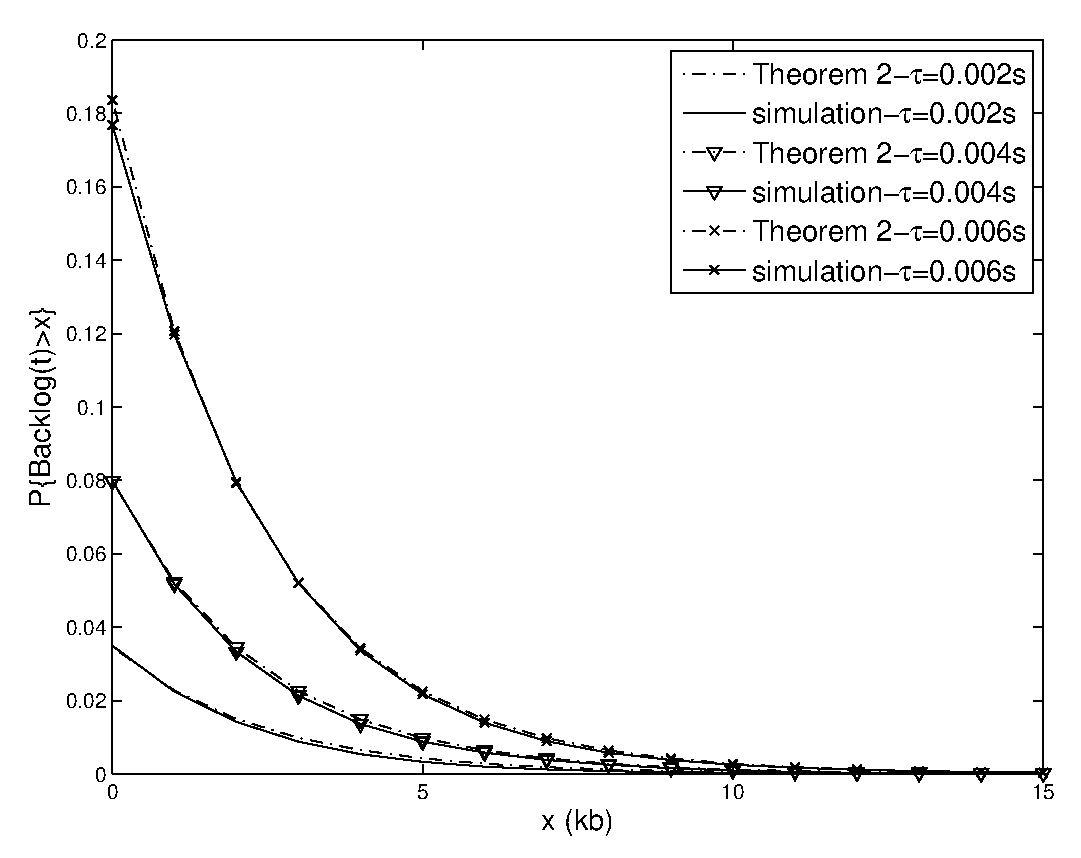
\includegraphics[scale=0.45]{figures/backlogtau.eps}\\
  \caption{Backlog Bound for Scenario I}\label{backlogtau}
\end{figure}

Set $L=1kb$, $C=1Mbps$, $\lambda=800s^{-1}$, $W=10kb$, and increasing the feedback delay $\tau$ from $0.002s$ to $0.006s$, we can get the simulation and numerical results, as shown in Fig. \ref{backlogtau}. The numerical results was conducted by selecting appropriated $\theta_1$ under the constraint of Eq.(\ref{stabilitycond2}) to make the right side of Eq.(\ref{bounding}) as small as possible. These comparisons indicate that, the backlog bound computed with Eq.(\ref{eqn2}) is very tight. Because a high efficient WFC can guarantee a lower blocking ratio at the controller, we can infer that, the efficiency of WFC increases while decreasing the feedback delay. To demonstrate this, continue to increase the feedback delay in this example, e.g. let $\tau=W\cdot \frac{L}{C}=0.01s$, the window flow controller will degenerated to a stop-and-wait flow control, which is of inefficiency.


\subsection{Scenario II}
In Subsection 3.3 of \cite{jung1996analysis}, the stationary probability $P\{\mathcal{L}=i\}$ was derived. Thus, the backlog bound can be calculated by
\begin{eqnarray}\label{oldresult}
P\{\mathcal{L}>x\}&=&\sum_{i=x+1}^\infty P\{\mathcal{L}=i\}\nonumber\\
&=& P(0,0)\rho^{(W+x+1)}/(1-\rho)
\end{eqnarray}
where $\rho=\lambda/\mu$ and $P(0,0)=1/(1+\sum_{i=1}^W\rho^i+\rho^{W+1}/(1-\rho))$.

Due to the independent and stationary properties of arrival and service process, we can apply Theorem \ref{theorem3} to obtain the follow backlog bound
\begin{equation}\label{newresult}
P\{\mathcal{L}>x\}\leq e^{-\theta(W+x)}e^{\lambda(e^{\theta L}-1)+\mu(e^{-\theta L}-1)}
\end{equation}
where $\theta$ satisfying $E[e^{\theta(\mathcal{A}(1)-\mathcal{S}(1))}]\leq 1$.

Let $\lambda=800s^{-1}$, $\mu=1000s^{-1}$, $\tau=0$ and $L=1kb$. We change the window size $W$ from $5kb$ to $15kb$, and present the numerical results calculated with Eq.(\ref{oldresult}) and Eq.(\ref{newresult}) in Fig. \ref{result3}. As shown in Fig. \ref{result3}, the backlog bound given in this paper is as tight as that given in \cite{jung1996analysis}, which is also the exact distribution of the backlog bound.
\begin{figure}
  \centering
  % Requires \usepackage{graphicx}
  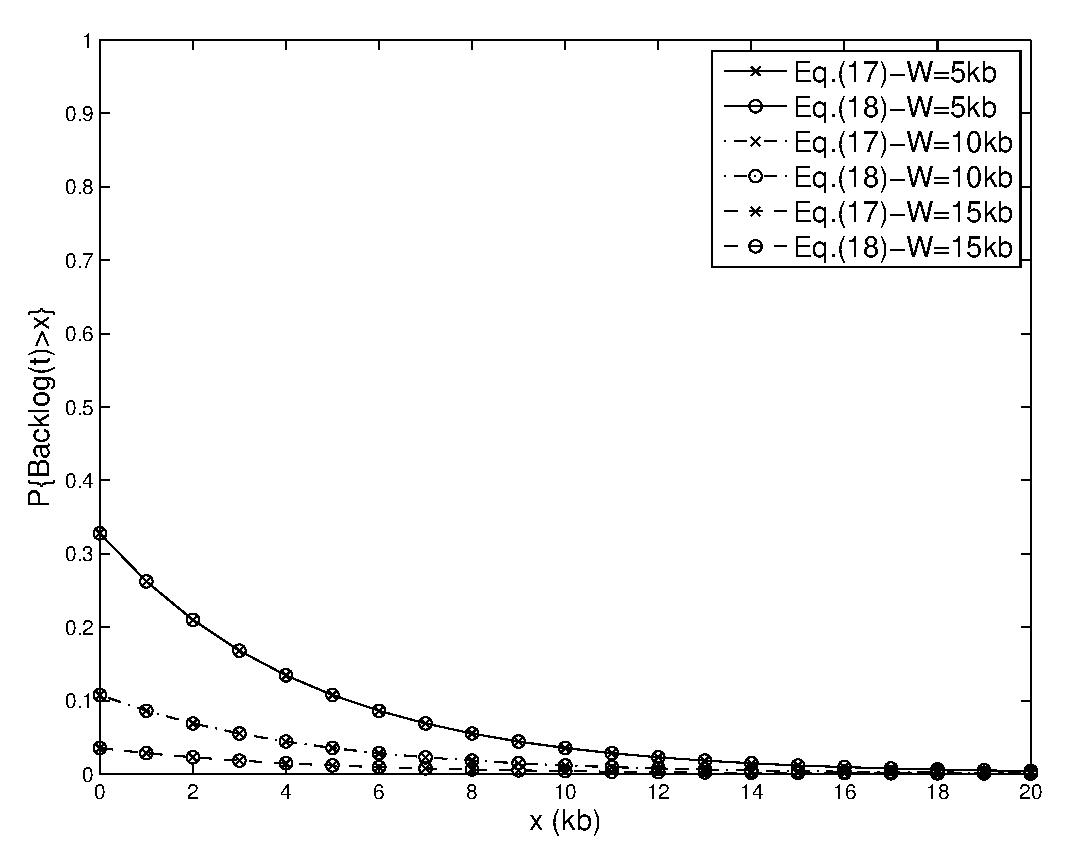
\includegraphics[scale=0.45]{figures/backlogcomp.eps}\\
  \caption{Backlog Bound for Scenario II}\label{result3}
\end{figure}

\subsection{Scenario III}
For this scenario, suppose the time is divided into slots with the same length $T$, and all the packets have the same length $L$. For each time slot, the source generates a packet with probability $p$ and keeps silent with probability $1-p$. Thus, arrival process $\mathcal{A}(t)$ is a typical two-states Markov-Modulated process, the effective bandwidth of this process can be found in \cite{Chan94}, i.e. $\rho(\theta)=\frac{1}{\theta}\log(1-p+pe^{\theta L})$. The effective capacity of the exponentially distributed service process with parameter $\mu$ is
\begin{eqnarray*}
\mu^\prime(\theta_2)&=& \frac{1}{-\theta_2}log E[e^{-\theta_2 \mathcal{S}(1)}]\\
&=& \frac{1}{-\theta_2}log(\sum_{x=0}^\infty e^{-\theta_2 Lx}\frac{e^{-\mu}\mu^x}{x!})\\
&=& \frac{\mu}{-\theta_2}(e^{-\theta_2 L}-1).
\end{eqnarray*}
\begin{figure}[tbp]
  \centering
  % Requires \usepackage{graphicx}
  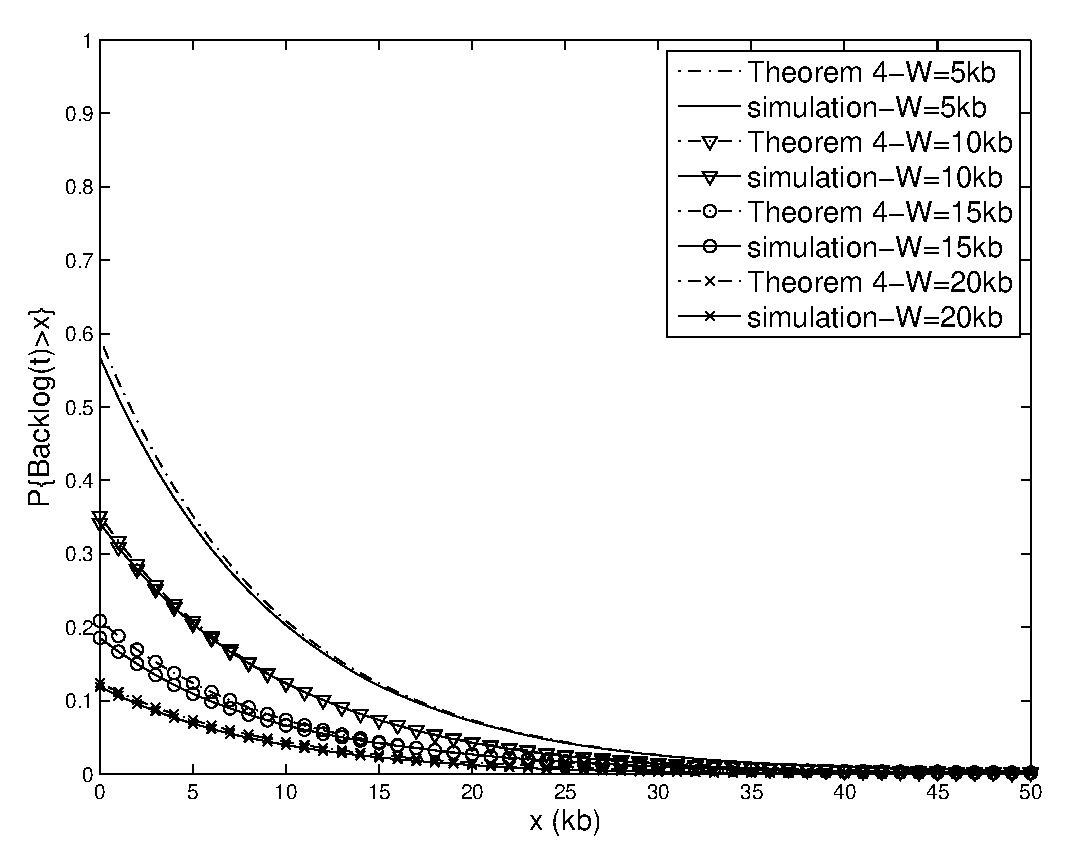
\includegraphics[scale=0.45]{figures/backlogbuf.eps}\\
  \caption{Backlog Bound for Scenario III with different Window Size}\label{result1}
\end{figure}
%The $v.b.c.$ stochastic arrival curve can be found in \cite{jiang2010note}, i.e. $<e^{-\theta_1\theta_1^\prime}e^{-\theta_1 x},\frac{t}{\theta_1}\log(1-p+pe^{\theta_1 L})+\theta_1^\prime t>$, where $\theta_1^\prime\geq 0$ and $\theta_1>0$ are free parameters.
%As stated in Theorem \ref{indstainc}, the independent and stationary service process has a $v.b.$ stochastic strict service curve $<e^{-\theta_2 x},\mu^\prime(\theta_2)\cdot t>$, where $\mu^\prime(\theta_2)\leq \frac{1}{-\theta_2}log E[e^{-\theta_2 \mathcal{S}(1)}]$. In this scenario, the service process provides exponentially distributed service time with parameter $\mu$ for each packet, and all the packets have some length $L$. Thus,
%Specifically, let $\mu^\prime(\theta_2)=\frac{\mu}{-\theta_2}(e^{-\theta_2 L}-1)$, we get a $v.b.$ stochastic strict service curve $<e^{-\theta_2 x},\frac{\mu}{-\theta_2}(e^{\theta_2 -L}-1)\cdot t>$.
%Let $\theta_1=\theta_2=\theta$, we get the following backlog bound
%\begin{eqnarray*}\label{backlogbounding}
%P\{\mathcal{L}(t)>x\}&\leq& 1-\bar{f}\ast\bar{g}([y^\prime]^+)\nonumber\\
%&=& e^{-\theta [y^\prime]^+}(1+\theta [y^\prime]^+ e^{-\theta_1^\prime \theta})
%\end{eqnarray*}
%where $y^\prime=x+W(t)-\alpha\oslash\beta(\tau)$. When applying Eq.(\ref{eqn2}) in this case, the following stability condition should be guaranteed
%\begin{equation*}\label{stabilitycond1}
%\frac{1}{\theta}(1-p+pe^{\theta L})+\frac{\mu}{\theta}(e^{-\theta L}-1)\leq 0.
%\end{equation*}
%We found that, the backlog bound computed with Eq.(\ref{eqn2}) for this scenario is not as tight as the previous one. In fact,

We can obtain the backlog bound with Theorem \ref{theorem2} or Theorem \ref{theorem3}, because the arrival and service processes of this scenario are both independent and stationary increment process. To demonstrate the tightness of Theorem \ref{theorem2} and Theorem \ref{theorem3}, we consider the follow two cases:

(1) $\tau=0$: We can obtain an backlog bound by applying Theorem \ref{theorem3}, which is
\begin{equation*}\label{equation3}
P\{\mathcal{L}(t)>x\}\leq e^{-\theta(W+x)}\cdot e^{\mu(e^{-\theta L}-1)+(1-p+pe^{\theta L})}
\end{equation*}
where $\theta>0$ and satisfying $\mu(e^{-\theta L}-1)+(1-p+pe^{\theta L})\leq 0$.

Let $L=1kb$, $\mu=40s^{-1}$, $T=0.02s$ and $W=5kb$, and change the window size from $5kb$ to $20kb$, we get the analytical results and simulation results. As shown in Fig. \ref{result1}, the analytical results match well with the simulation results. Another observation is that, the backlog bound decreases along with the increasing of window size. However, the larger window size, the larger risk of network congestion. This indicates that, there is a tradeoff between the efficiency of flow control and the cost of network congestion.

(2) $\tau> 0$: For this scenario, both of the arrival and service process are stationary, thus, we can get a backlog bound by applying Theorem \ref{theorem2}, which is
\begin{equation}\label{bernoullibound}
P\{\mathcal{L}(t)>x\}\leq e^{-\theta [x+W-\rho(\theta)\cdot \tau]}.
\end{equation}
This backlog bound can be minimized by selecting free parameters $\theta$ satisfying the following stability condition
\begin{equation}\label{stabilitycond3}
\rho(\theta)\leq \mu^\prime(\theta).
\end{equation}

Set $L=1kb$, $T=0.02s$, $W=5kb$, $\mu=50s^{-1}$ and $\tau=0.002s$, we change the offered load by increasing the probability $p$ from $0.8$ to $0.95$. The simulation and numerical results are shown in Fig. \ref{result2}. The numerical results was conducted by selecting appropriate $\theta$ under the constraint of Eq.(\ref{stabilitycond3}) to make the Eq.(\ref{bernoullibound}) as small as possible. As shown in the Fig. \ref{result2}, the backlog bounds match well with the simulation results, which indicates that, our theoretical bounds based on SNC can indeed predicating the performance of WFC exactly.
\begin{figure}[tbp]
  \centering
  % Requires \usepackage{graphicx}
  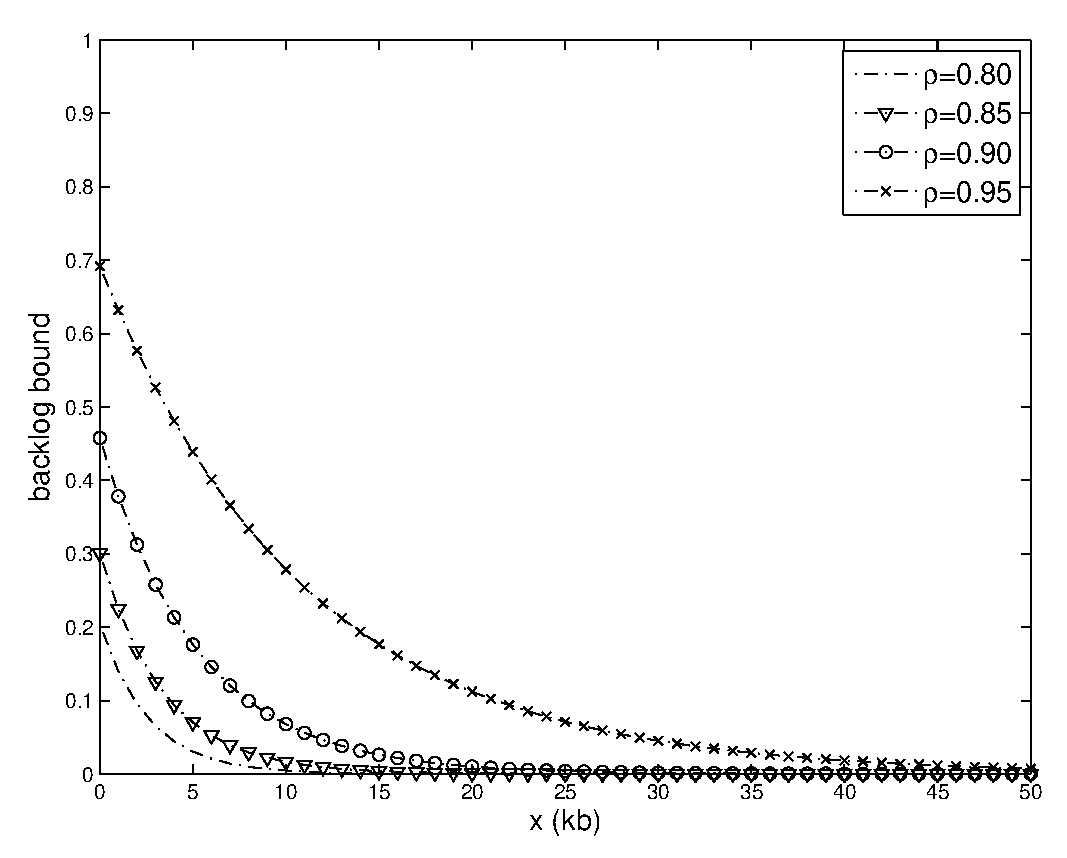
\includegraphics[scale=0.45]{figures/backlogrho.eps}\\
  \caption{Backlog Bound for Scenario III with different Offered Load}\label{result2}
\end{figure}

\section{Conclusion}\label{concluson}
Flow control has been widely used in the computer network to avoid network congestion, deadlock and unfair resource allocation. In this paper, we proposed a Stochastic Network Calculus (SNC) based performance model to evaluate the backlog bound of lossless Window Flow Controller (WFC). The derivation is conducted by leveraging the concept of beginning of last backlogged period and some advanced probability techniques, e.g. effective bandwidth, effective capacity and martingale. Given the WFC parameters (i.e. feedback delay and window size) and the traffic and service characterizations, our analytical framework can answer question related to the backlog bound of the controller. Our work is not only the stochastic extension for the previous research on the performance analysis of WFC with deterministic network calculus, but also the generalization of the existing queueing theory based performance model. In addition, the influence of different WFC parameters on the backlog bound are also investigated. In the future work, we expect to extend these results to support the hop-by-hop window flow control.

\section*{Acknowledgment}
The authors would thank the reviewers for their suggestions and comments, and the first author would thanks Prof. Yuming Jiang of Norwegian University of Science and Technology (NTNU) for the fruitful discussion on the stochastic network calculus theory. This research is supported by High Technology Research and Development Program of China (Grant No. 2012AA012201, 2012AA011902).

\bibliographystyle{ieicetr}% bib style
\bibliography{Docear}% your bib database

%\begin{thebibliography}{99}% more than 9 --> 99 / less than 10 --> 9
%\bibitem{}
%\end{thebibliography}

\profile[figures/me.eps]{Baoliang Li}{ was born in 1987. He received the B.S. degree in Computer Science and Technology from Tsinghua University, P.R. China, in 2009. He is currently working towards the Ph.D. degree from College of Computer at National University of Defense Technology (NUDT), P.R. China. His research interests is performance analysis of computer networks and Networks-on-Chip, with a special interest on the analytical methods of network calculus.}
\profile[figures/zj.eps]{Jie Zhao}{was born in 1987. He receive the B.S. degree from Tsinghua University (Beijing, 100084, P. R. China) in Sep. 2009 and the M.S. degree in State Key Laboratory of Mathematical Engineering and Advanced Computing in 2012. He is currently working toward the Ph.D. degree in State Key Laboratory of Mathematical Engineering and Advanced Computing, Wuxi, 214125, P.R. China. His research focuses on parallel computing and computer networks.}
\profile[figures/dwh.eps]{Wenhua Dou}{ was born in 1946. He received the B.S. degree in computer science from Harbin Military Engineering College in 1970. He has been working at National University of Defense Technology (NUDT), P.R. China since 1970. He was vice dean of College of Computer, NUDT from 1999 to 2003. He is currently a professor of College of Computer, NUDT with research focusing on computer networks.}
%\profile*{}{}% without picture of author's face

\end{document}
